
\begin{tframe}{Face Detector}
\begin{tabular}{cl}  
\begin{tabular}{l}
\parbox{0.5\linewidth}{%  change the parbox width as appropiate

The next phases have the objective of \textbf{filtering} the obtained dataset, in order to remove, for each identity, the images that are not relevant. 

\vspace{0.1in}

The results of the queries to the image search engines for a specific identity, will also contain images that are not related to that identity, thus the need of a filtering phase. 

\vspace{0.1in}

Since the objective of this paper is the creation of datasets of images containing \textbf{faces}, we need to detect and select the faces in the retrieved images.

}
\end{tabular} & \begin{tabular}{c}
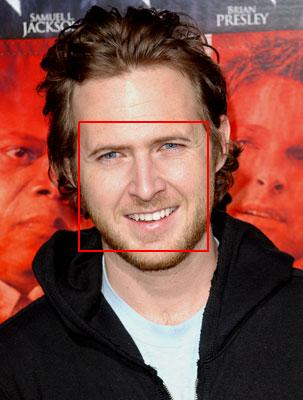
\includegraphics[height=5cm, width=3.5cm]{images/image3.jpg}
\end{tabular}  \\
\end{tabular}
\end{tframe}


\begin{tframe}{Face Detector}

This task is accomplished implementing a \textbf{face detector}, written in C++ using the \textbf{Dlib} library [2]. 

\vspace{0.1in}

The \textbf{Dlib} C++ library implements a face detector by using the classic \textbf{histogram of oriented gradients} (\textbf{HOG}) feature combined with a linear classifier, an image pyramid and sliding window detection scheme.

\vspace{0.1in}

The face detector takes an image, or list of images, and returns the coordinates of the \textbf{bounding box} surrounding the detected faces, which are then saved in the database.

\begin{figure}[h]
\begin{center}
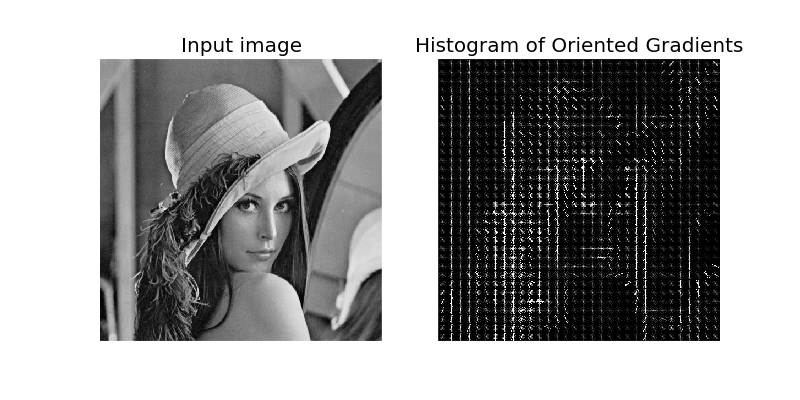
\includegraphics[width=0.7\textwidth]{images/hog.png}
\end{center}
\end{figure}

\end{tframe}